\documentclass[fleqn]{article}
\usepackage[margin=1in]{geometry}
\usepackage[nodisplayskipstretch]{setspace}
\usepackage{amsmath, nccmath, bm}
\usepackage{amssymb}
\usepackage{enumitem}
\usepackage{graphicx}
\usepackage{float}
\usepackage{listings}
\usepackage{hyperref}
\usepackage[svgnames]{xcolor}
\usepackage{indentfirst}
%\usepackage{chngcntr}
%\counterwithin{table}{section}
\graphicspath{
{./images}
{./images/nand}
{./images/nand/delay}
{./images/nand/design}
{./images/nand/noise_analysis}
{./images/nand/power}
{./images/nand/vtc}
{./images/nor}
{./images/nor/delay}
{./images/nor/design}
{./images/nor/noise_analysis}
{./images/nor/power}
{./images/nor/vtc}}

\hypersetup{
    colorlinks=true,
    linkcolor=black,
    filecolor=black,      
    urlcolor=blue
    }

\newcommand{\zerodisplayskip}{
	\setlength{\abovedisplayskip}{0pt}%
	\setlength{\belowdisplayskip}{0pt}%
	\setlength{\abovedisplayshortskip}{0pt}%
	\setlength{\belowdisplayshortskip}{0pt}%
	\setlength{\mathindent}{0pt}}
	
\definecolor{vgreen}{RGB}{104,180,104}
\definecolor{vblue}{RGB}{49,49,255}
\definecolor{vorange}{RGB}{255,143,102}

\lstdefinestyle{verilog-style}
{
    language=Verilog,
    basicstyle=\small\ttfamily,
    keywordstyle=\color{vblue},
    identifierstyle=\color{black},
    commentstyle=\color{vgreen},
    numbers=left,
    numberstyle=\tiny\color{black},
    numbersep=10pt,
    tabsize=8,
    moredelim=*[s][\colorIndex]{[}{]},
    literate=*{:}{:}1
}

\lstset{style={verilog-style},showstringspaces=false}

\makeatletter
\newcommand*\@lbracket{[}
\newcommand*\@rbracket{]}
\newcommand*\@colon{:}
\newcommand*\colorIndex{%
    \edef\@temp{\the\lst@token}%
    \ifx\@temp\@lbracket \color{black}%
    \else\ifx\@temp\@rbracket \color{black}%
    \else\ifx\@temp\@colon \color{black}%
    \else \color{vorange}%
    \fi\fi\fi
}
\makeatother

\newcommand{\code}[1]{%
	\colorbox{Gainsboro}{\texttt{#1}}%
}

\title{Lab 1}
\author{Owen Sowatzke}
\date{March 17, 2025}

\begin{document}

	% \offinterlineskip
	% \setlength{\lineskip}{12pt}
	% \zerodisplayskip
	\maketitle
	
	\section{Introduction}
	
	\section{Procedure}
	
	\section{Results}
	
	\subsection{First Order Transistor Model}
	
	\texttt{let ids=-vds\#branch}
	
	\texttt{let ids\_p=deriv(ids)}
	
	\texttt{plot ids\_p}
	
	\texttt{let ids\_pp=deriv(ids\_p)}
	
	\texttt{meas dc m max ids\_pp}
	
	\texttt{meas dc vgs\_i max\_at ids\_pp}
	
	\texttt{meas dc ids\_p\_i find ids\_p when vgs=vgs\_i}
	
	\texttt{let b = ids\_p\_i - m*vgs\_i}
	
	\texttt{let vt = -b/m}
	
	\texttt{print vt}
	
	\texttt{let ids\_p\_fit = m*vgs + b}
	
	\texttt{plot ids\_p ids\_p\_fit yrange}
	
	\begin{center}
	\label{table::nmos_params}
	\begin{tabular}{| c | c |}
		\hline
		Parameter & Value \\
		\hline	
		$V_{t0}$ & $0.6613 V$\\
		\hline	
		$V_{dsat}$ & $0.3948 V$\\
		\hline	
		$\lambda$ & $0.1289 V^{-1}$\\
		\hline			
		$k_n$ & $164.1 {\mu}A/V^2$ \\
		\hline
	\end{tabular}
	\end{center}
	
	\begin{center}
	\begin{tabular}{| c | c |}
		\hline
		Parameter & Value \\
		\hline	
		$V_{t0}$ & $-0.5765 V$\\
		\hline	
		$V_{dsat}$ & $-0.7988 V$\\
		\hline	
		$\lambda$ & $-0.3408 V^{-1}$\\
		\hline			
		$k_n$ & $28.48 {\mu}A/V^2$ \\
		\hline
	\end{tabular}
	\end{center}
	
	\begin{table}
	\begin{center}
	\caption{Inputs that Create High to Low Transition for NOR Gate}
	\begin{tabular}{| c | c |}
		\hline
		\texttt{a} & \texttt{b} \\
		\hline	
		$0 \rightarrow 1$ & $0$\\
		\hline	
		$0$ & $0 \rightarrow 1$\\
		\hline	
		$0 \rightarrow 1$ & $0 \rightarrow 1$\\
		\hline
	\end{tabular}
	\end{center}
	\end{table}
	
	\subsection{NAND Gate}
	
	\subsubsection{Design}
	
	The NAND gate pull-down circuit is composed of two NMOS transistors in series. The pull-up circuit is the complement of the pull-down circuit and is composed of two parallel PMOS transistors. For analysis, we can create an equivalent inverter from the NAND gate. In this equivalent inverter, the channel length of the NMOS transistor is doubled because the NMOS transistors in the NAND gate are laid out in series. (This is equivalent to halving the width of the transistor). The NAND gate pull-up circuit is on when either transistor is on. However, for analysis, we consider the worst (slowest) case, when only one transistor is on. Therefore, the PMOS transistor width in the equivalent inverter remains unchanged.
	
	For an inverter, we know that we need to make the width of the PMOS transistor twice as large as the width NMOS transistor because the mobility of holes is lower than the mobility of electrons. We can map these sizes back to the NAND gate. Doing so, we find that PMOS transistor width in the NAND gate should be the same as the inverter, and the NMOS transistor width should be doubled. To match the behavior of the inverter with a NMOS width of 1 and a PMOS width of 2, we should make the NMOS width 2 and the PMOS width 2. The NAND gate circuit with these transistor widths is shown in Figure \ref{fig::nand_schematic}.
	
	\begin{figure}[H]
		\centerline{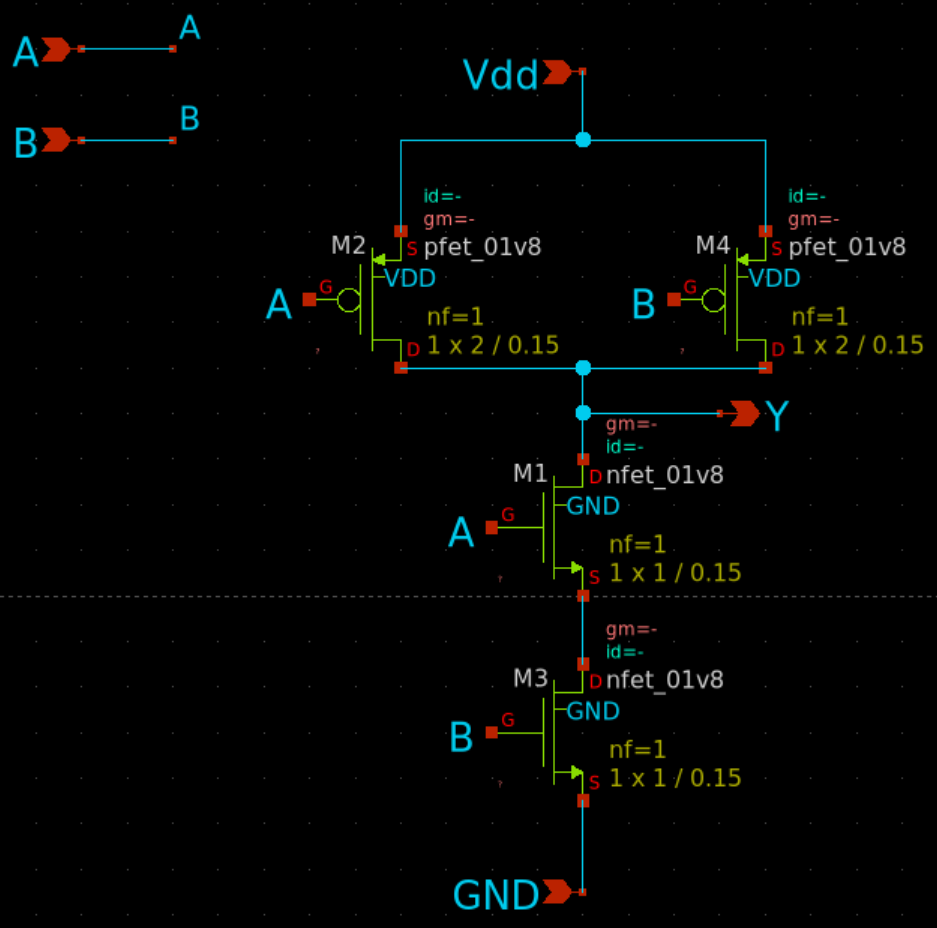
\includegraphics[width=0.4\textwidth]{nand_schematic.png}}
		\caption{NAND Circuit Schematic}
		\label{fig::nand_schematic}
	\end{figure}

	\noindent We also create a circuit symbol for the NAND gate, to allow reuse in other schematics. This circuit symbol is shown in Figure \ref{fig::nand_symbol}.
	
	\begin{figure}[H]
		\centerline{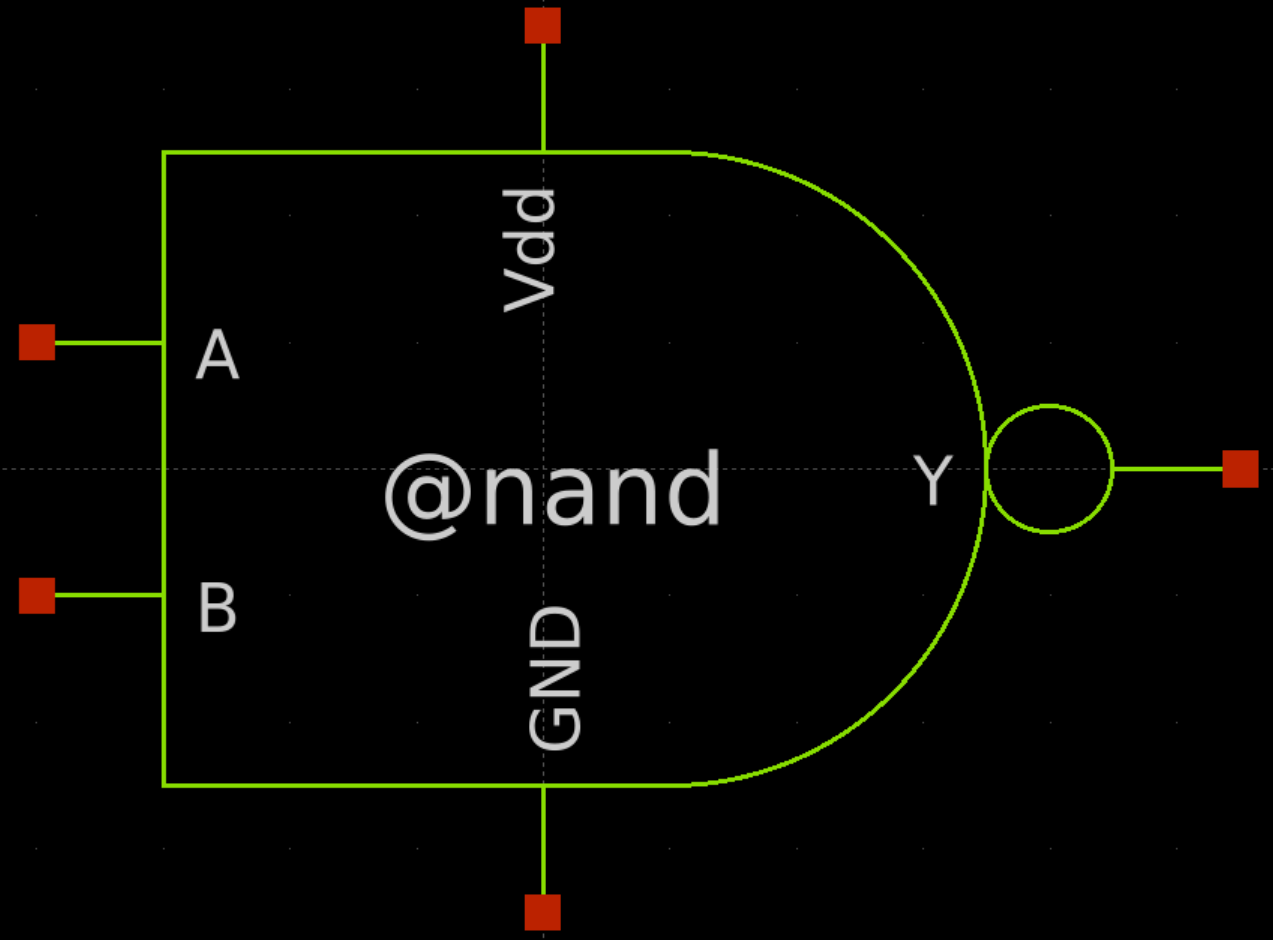
\includegraphics[width=0.4\textwidth]{nand_symbol.png}}
		\caption{NAND Circuit Symbol}
		\label{fig::nand_symbol}
	\end{figure}
	
	\subsubsection{Voltage Transfer Characteristics}
	
	In this section, we analyze the voltage transfer characteristics (VTC) of our NAND gate. For this analysis, we need to analyze the VTC for all combinations of inputs that lead to a logic level change. To generate the VTC in ngspice, we only need to consider one set of transitions because we care about the steady state output voltages for each input voltage. As such, we analyze the input voltages that result in high-to-low transitions. These voltages are dictated in Table \ref{table::nand_gate_high_to_low_transitions}.
	
	\begin{table}[H]
	\begin{center}
	\caption{Inputs that Create High to Low Transition for NAND Gate}
	\label{table::nand_gate_high_to_low_transitions}
	\begin{tabular}{| c | c |}
		\hline
		\texttt{a} & \texttt{b} \\
		\hline	
		$0 \rightarrow 1$ & $1$\\
		\hline	
		$1$ & $0 \rightarrow 1$\\
		\hline	
		$0 \rightarrow 1$ & $0 \rightarrow 1$\\
		\hline
	\end{tabular}
	\end{center}
	\end{table}
	
	\noindent The test circuit we use to generate the VTC for the first entry in the above table is shown in Figure \ref{fig::nand_vtc_test_sweep_va}.
	
	\begin{figure}[H]
		\centerline{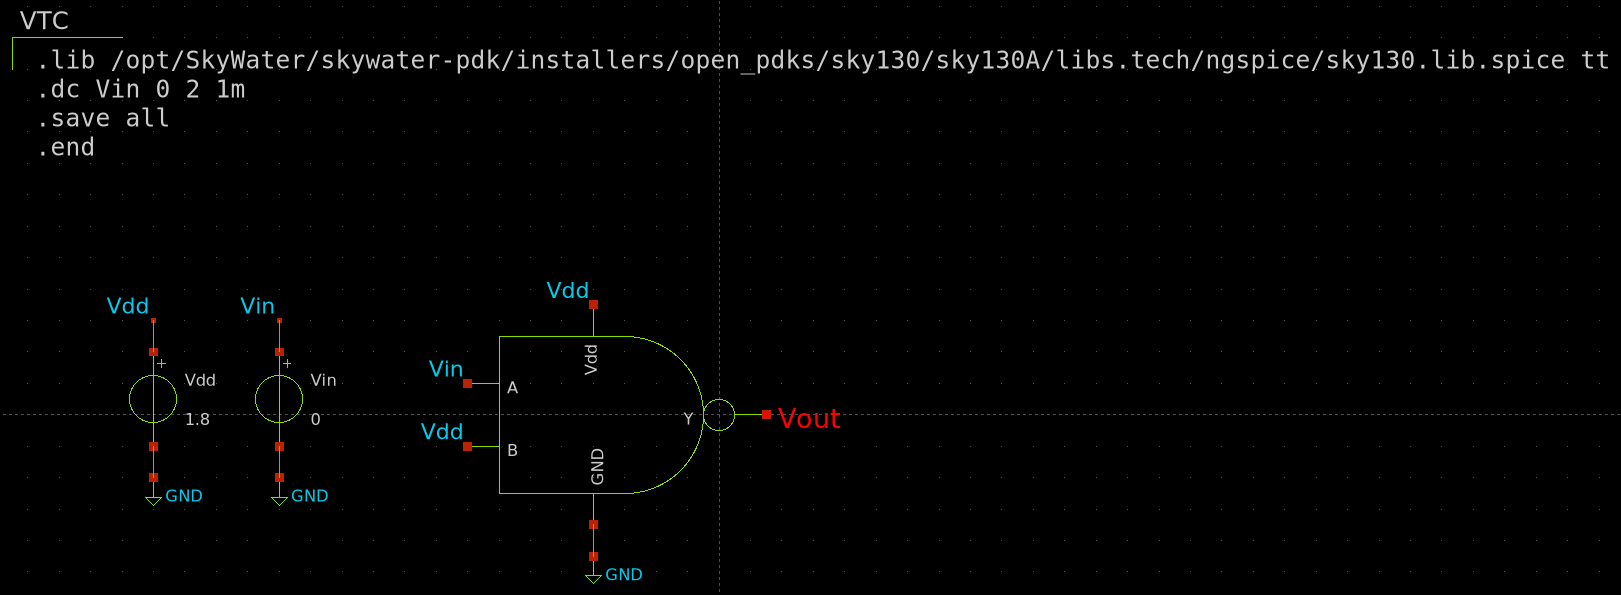
\includegraphics[width=0.8\textwidth]{nand_vtc_test_sweep_va.png}}
		\caption{NAND VTC Test Circuit for Variations of \texttt{a} with \texttt{b=1}}
		\label{fig::nand_vtc_test_sweep_va}
	\end{figure}	
	
	\noindent Using this test circuit, we perform DC analysis to generate the VTC and find \texttt{Vm}, which is the voltage at which \texttt{Vin = Vout}. The results of this analysis are shown in Figure \ref{fig::nand_vtc_sweep_va}.
	
	\begin{figure}[H]
		\centerline{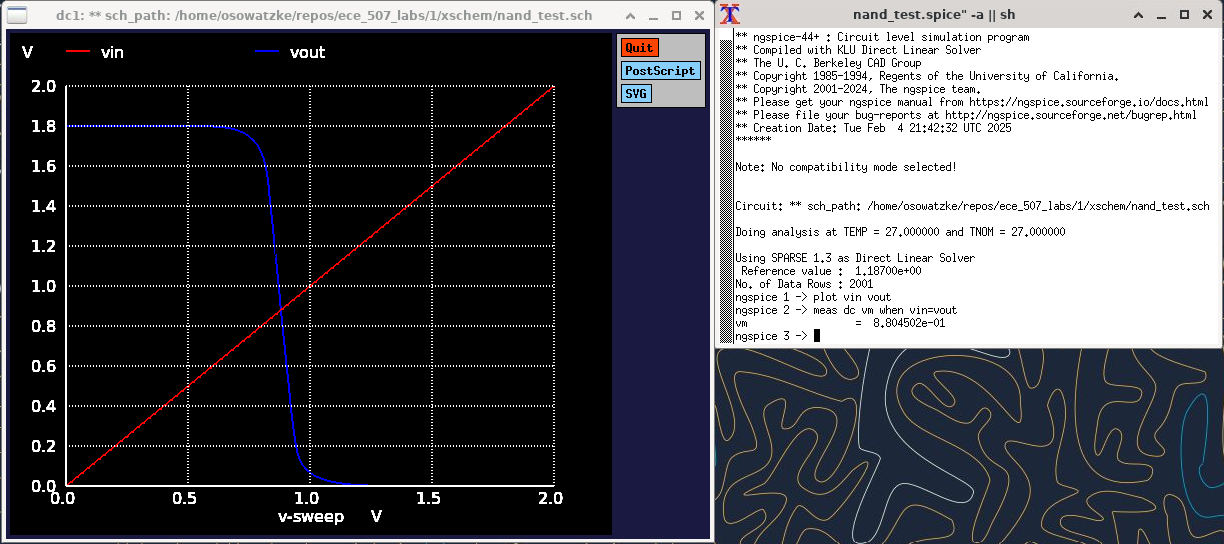
\includegraphics[width=0.8\textwidth]{nand_vtc_sweep_va.png}}
		\caption{NAND VTC Results for Variations of \texttt{a} with \texttt{b=1}}
		\label{fig::nand_vtc_sweep_va}
	\end{figure}
	
	Examining the results, we find that \texttt{Vm = 0.8257V}. With slight modifications to our test circuit, we perform similar analysis to find \texttt{Vm} for the other sets inputs listed in Table \ref{table::nand_gate_high_to_low_transitions}. These results are included in Table \ref{table::nand_gate_vm}.
	
	\begin{table}[H]
	\begin{center}
	\caption{\texttt{Vm} for Each Set of Inputs That Result in an Output Logic Level Change}
	\label{table::nand_gate_vm}
	\begin{tabular}{| c | c | c |}
		\hline
		\texttt{a} & \texttt{b} & \texttt{Vm}\\
		\hline	
		$0 \rightarrow 1$ & $1$ & $0.8257 \text{V}$\\
		\hline	
		$1$ & $0 \rightarrow 1$ & $0.8195 \text{V}$\\
		\hline	
		$0 \rightarrow 1$ & $0 \rightarrow 1$ & $0.9108 \text{V}$\\
		\hline
	\end{tabular}
	\end{center}
	\end{table}
	
	\noindent Reviewing our captured results, we see that \texttt{Vm} is dependent on the gate inputs. \texttt{Vm} is the largest when both gates switch at the same time. This makes sense because our pull-up network is strongest in this case, causing \texttt{Vm} to shift to the right.
	
	\subsubsection{Noise Analysis}
	\label{section::nand_noise_analysis}
	
	Using the test circuit shown in Figure \ref{fig::nand_vtc_test_sweep_va}, we can also measure the noise margins, which are defined follows:
	
	\begin{equation}
		NM_H = V_{OH} - V_{IH}
		\label{eq::noise_margin_high}
	\end{equation}
	
	\begin{equation}
		NM_L = V_{IL} - V_{OL}
		\label{eq::noise_margin_low}
	\end{equation}
	
	In the above formulas, $V_{IH}$ and $V_{IL}$ are defined as the unity points of the gain function, where the gain is defined as the derivative of the VTC. For the case in which we vary \texttt{a} with \texttt{b=1}, we can identify the unity gain points and solve for the noise margins.
	
	\begin{figure}[H]
		\centerline{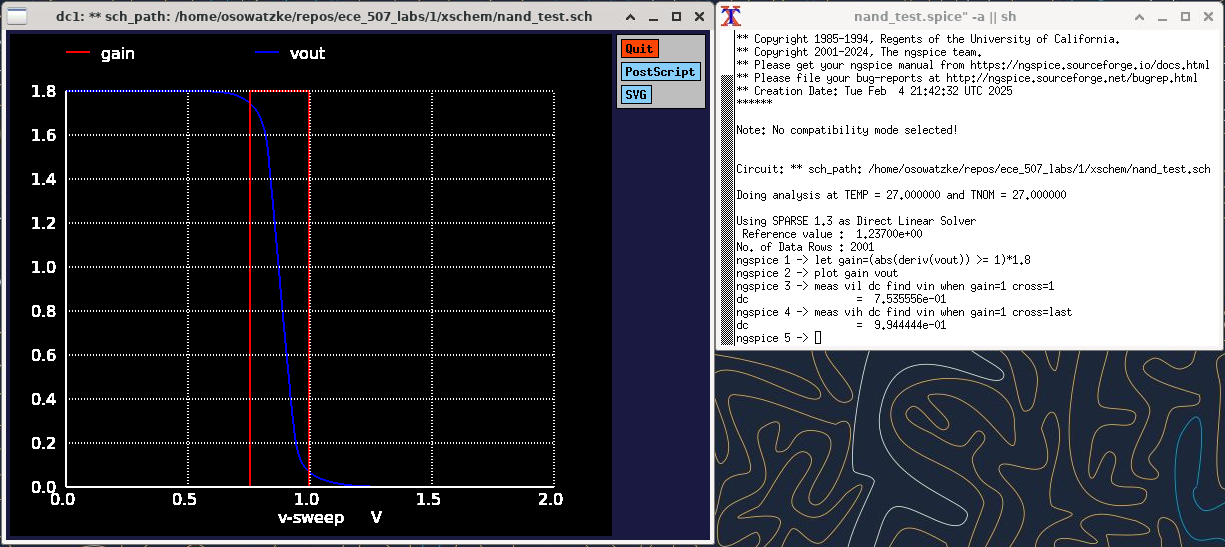
\includegraphics[width=0.8\textwidth]{nand_noise_analysis_sweep_va.png}}
		\caption{Measuring Noise Margins for the NAND Gate when \texttt{a} is Varied and \texttt{b=1}}	\label{fig::nand_noise_analysis_sweep_va}
	\end{figure}
	
	Examining the outputs shown in Figure \ref{fig::nand_noise_analysis_sweep_va}, we find that \texttt{Vil = 0.6926 V} and \texttt{Vih = 0.9264 V}. This implies that \texttt{Nmh = 1.8 V - 0.9264 V = 0.8736 V} and \texttt{Nml = 0.6926 V - 0 V = 0.6926 V}. With slight modifications to the test circuit, we can measure the noise margins for the sets of inputs listed in Table \ref{table::nand_gate_high_to_low_transitions}. Our results for this analysis are listed in Table \ref{table::nand_gate_noise_analysis}.
	
	\begin{table}[H]
	\begin{center}
	\caption{Noise Margins for Each Set of Inputs That Result in an Output Logic Level Change}
	\label{table::nand_gate_noise_analysis}
	\begin{tabular}{| c | c | c | c | c | c |}
		\hline
		\texttt{a} & \texttt{b} & \texttt{Vih} & \texttt{Vil} & \texttt{Nmh} & \texttt{Nml} \\
		\hline	
		$0 \rightarrow 1$ & $1$ & $0.9264 \text{V}$ & $0.6926 \text{V}$ & $0.8736 \text{V}$ & $0.6926 \text{V}$\\
		\hline	
		$1$ & $0 \rightarrow 1$ & $0.9184 \text{V}$ & $0.7116 \text{V}$ & $0.8816 \text{V}$ & $0.7116 \text{V}$\\
		\hline	
		$0 \rightarrow 1$ & $0 \rightarrow 1$ & $1.0224 \text{V}$ & $0.8046 \text{V}$ & $0.7776 \text{V}$ & $0.8046 \text{V}$\\
		\hline
	\end{tabular}
	\end{center}
	\end{table}
	
	\subsubsection{Delay Analysis}
	
	In this section, we analyze the propagation delay of the NAND gate. To do so, we need to measure both the high-to-low propagation delay (\texttt{tphl}) and the low-to-high propagation delay. We measure \texttt{tphl} for each of the transitions listed in Table \ref{table::nand_gate_high_to_low_transitions}, and we measure \texttt{tplh} for each of the transitions listed in Table \ref{table::nand_gate_low_to_high_transitions}.
	
	\begin{table}[H]
	\begin{center}
	\caption{Inputs that Create Low-to-High Transition for NAND Gate}
	\label{table::nand_gate_low_to_high_transitions}
	\begin{tabular}{| c | c |}
		\hline
		\texttt{a} & \texttt{b} \\
		\hline	
		$1 \rightarrow 0$ & $1$\\
		\hline	
		$1$ & $1 \rightarrow 0$\\
		\hline	
		$1 \rightarrow 0$ & $1 \rightarrow 0$\\
		\hline
	\end{tabular}
	\end{center}
	\end{table}
	
	\noindent For variations of \texttt{a} with \texttt{b=1}, we can use the test circuit shown in Figure \ref{fig::nand_delay_test_sweep_va} to measure propagation delays. Note the input waveforms contains both rising an falling edges, so we can use it to measure \texttt{tphl} and \texttt{tplh}.

	\begin{figure}[H]
		\centerline{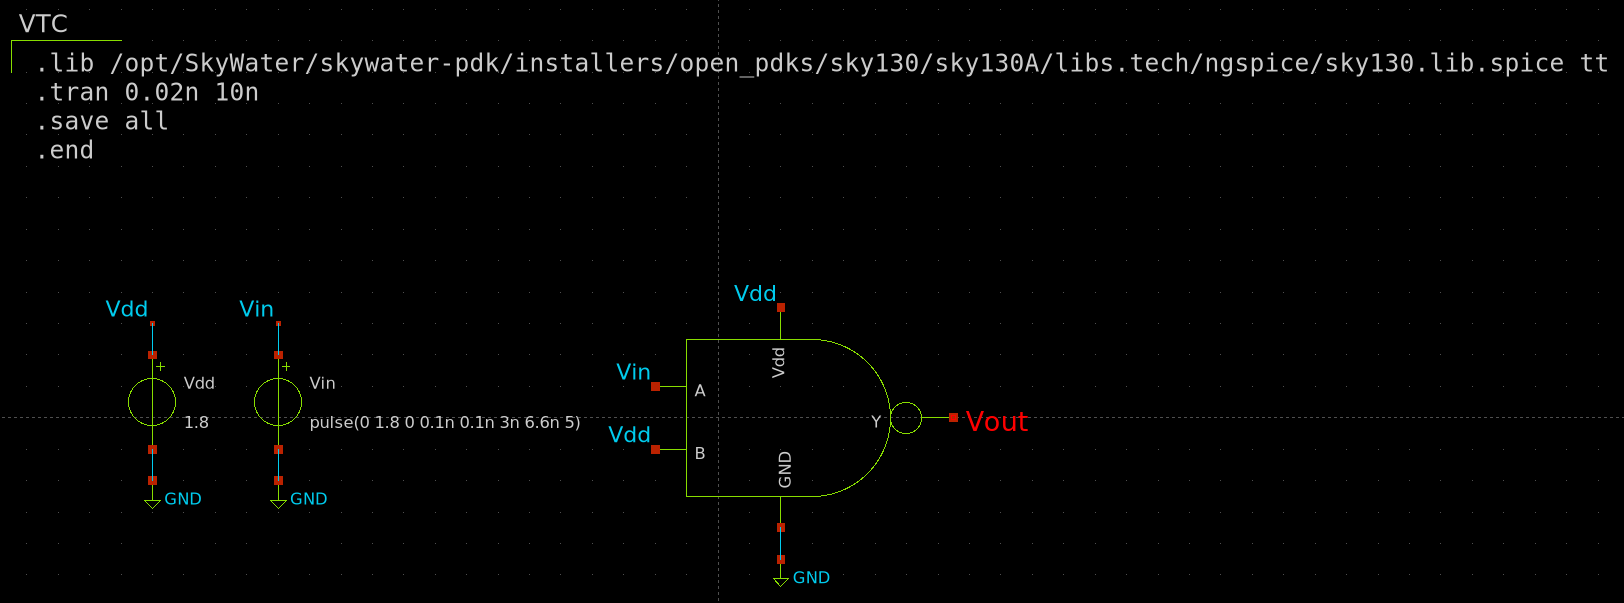
\includegraphics[width=0.8\textwidth]{nand_delay_test_sweep_va.png}}
		\caption{Test Circuit to Measure the Delay of the NAND Gate when \texttt{a} is Varied and \texttt{b=1}}
		\label{fig::nand_delay_test_sweep_va}
	\end{figure}
	
	\noindent Using the test circuit, we measure can measure \texttt{tphl} and \texttt{tplh} as follows:
	
	\begin{figure}[H]
		\centerline{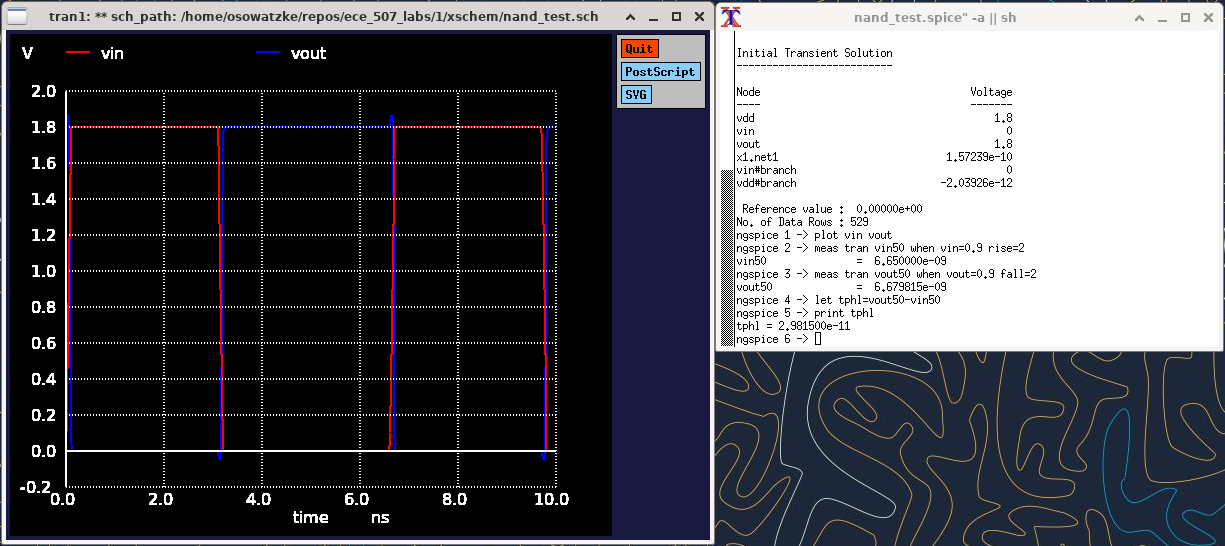
\includegraphics[width=0.8\textwidth]{nand_delay_sweep_va.png}}
		\caption{\texttt{tphl} Measurement for the NAND Gate when \texttt{a} is Varied and \texttt{b=1}}
		\label{fig::nand_delay_sweep_va}
	\end{figure}
	
	Examining the output results, we find that \texttt{tphl = 20.859 ps} for \texttt{a = }$0 \rightarrow 1$ and \texttt{b = 1}. Similarly, we find that \texttt{tphl = 33.178 ps} for \texttt{a = }$1 \rightarrow 0$ and \texttt{b = 1}. We perform similar analysis for the remaining transitions listed in Table \ref{table::nand_gate_high_to_low_transitions} and Table \ref{table::nand_gate_high_to_low_transitions}. Our results are summarized in Table \ref{table::nand_gate_delay_analysis}.
	
	\begin{table}[H]
	\begin{center}
	\caption{Propagation Delays for Each Transition That Result in an Output Logic Level Change}
	\label{table::nand_gate_delay_analysis}
	\begin{tabular}{| c | c | c || c | c | c |}
		\hline
		\texttt{a} & \texttt{b} & \texttt{tphl} & \texttt{a} & \texttt{b} & \texttt{tplh} \\
		\hline	
		$0 \rightarrow 1$ & $1$ & $20.859\ \text{ps}$ & $1 \rightarrow 0$ & $1$ & $33.178\ \text{ps}$\\
		\hline	
		$1$ & $0 \rightarrow 1$ & $28.146\ \text{ps}$ & $1$ & $1 \rightarrow 0$ & $48.137\ \text{ps}$\\
		\hline	
		$0 \rightarrow 1$ & $0 \rightarrow 1$ & $29.297\ \text{ps}$ & $1 \rightarrow 0$ & $1 \rightarrow 0$ & $26.097\ \text{ps}$\\
		\hline
	\end{tabular}
	\end{center}
	\end{table}
	
	\subsubsection{Power Analysis}
	
	In this section, we analyze the power consumption of our NAND gate. Similar to what we did above, we analyze the power consumption for each input variation that results in an output logical level change. For our input, we used a pulsed source. This allows us to capture both rising and falling edges of the output. We use the test circuit shown in Figure \ref{fig::nand_power_test_sweep_va} to measure the power consumption for variations of \texttt{a} with \texttt{b=1}. For this analysis, we have also attached a parasitic capacitance to the gate output.
	
	\begin{figure}[H]
		\centerline{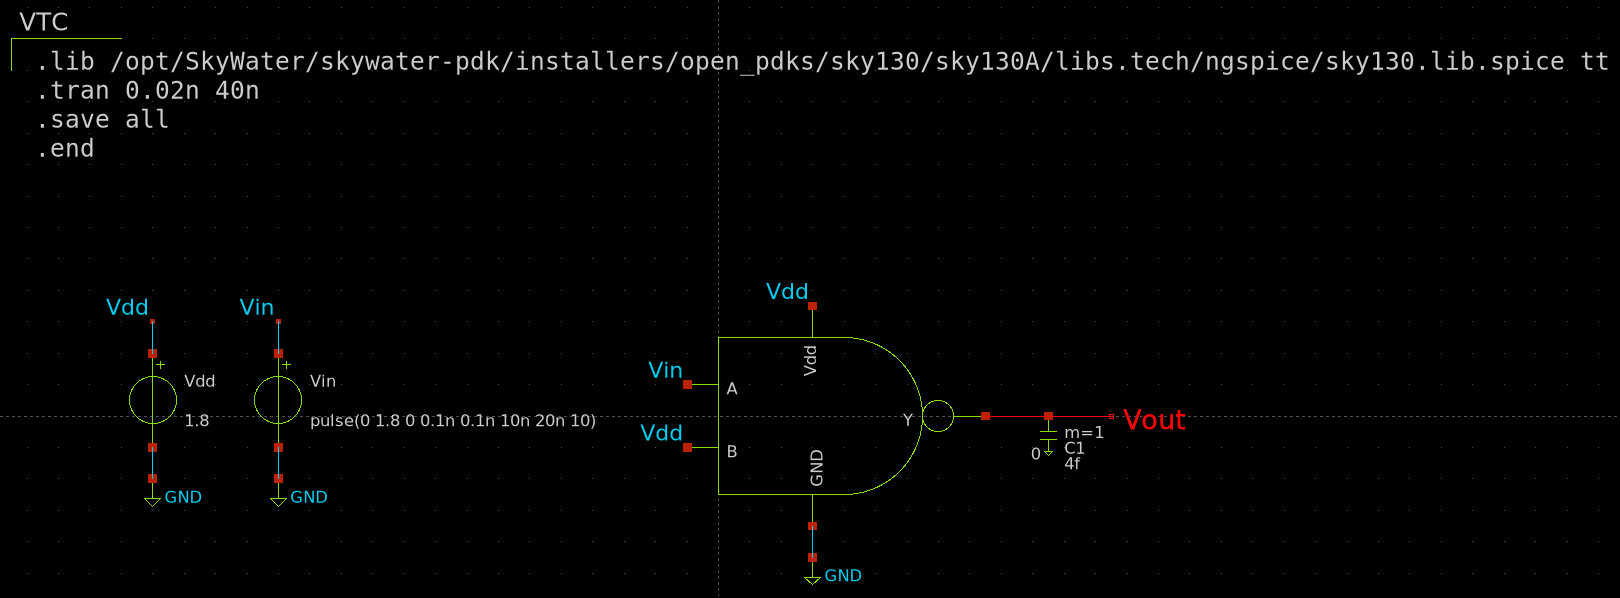
\includegraphics[width=0.8\textwidth]{nand_power_test_sweep_va.png}}
		\caption{Test Circuit to Measure the Power Consumption of the NAND Gate when \texttt{a} is Varied and \texttt{b=1}}
		\label{fig::nand_power_test_sweep_va}
	\end{figure}
	
	\noindent Using the test circuit, we measure the power consumption as follows:
	
	\begin{figure}[H]
		\centerline{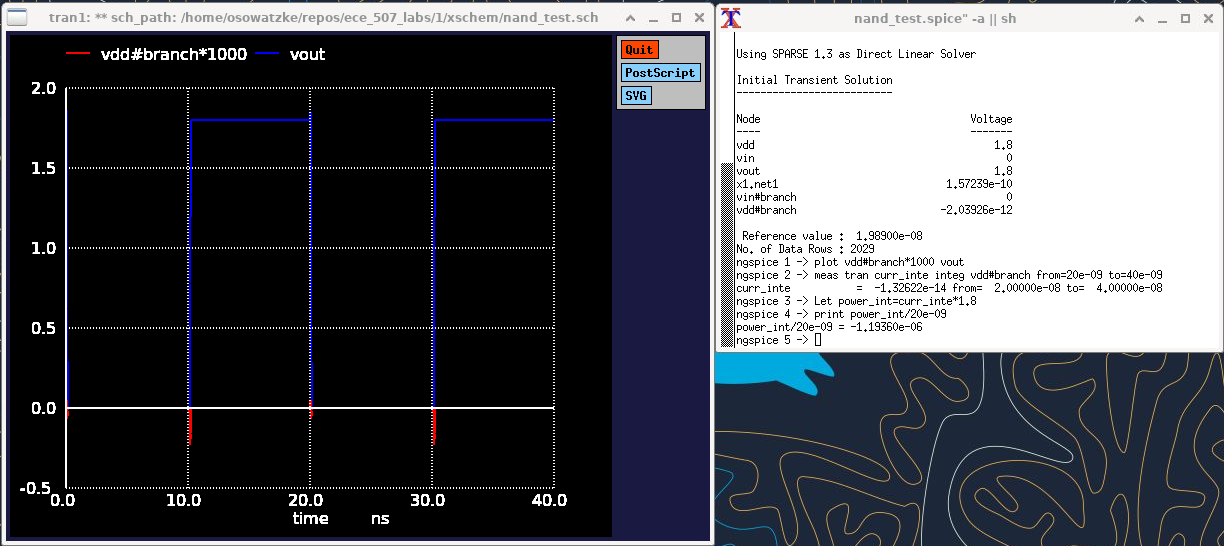
\includegraphics[width=0.8\textwidth]{nand_power_sweep_va.png}}
		\caption{Power Consumption of the NAND Gate when \texttt{a} is Varied and \texttt{b=1}}
		\label{fig::nand_power_sweep_va}
	\end{figure}
	
	\noindent Examining the results, we find that the power consumption is $1.34880{\mu}W$. Note that this power estimate includes the effects of the rising and falling edges of \texttt{a}. We can perform similar analysis for other variations of the input. Our results for this work are summarized in Table \ref{table::nand_gate_power_analysis}.
	
	\begin{table}[H]
	\begin{center}
	\caption{NAND Gate Power Consumption for Different Input Variations}
	\label{table::nand_gate_power_analysis}
	\begin{tabular}{| c | c | c |}
		\hline
		\texttt{a} & \texttt{b} & \texttt{Power}\\
		\hline	
		$0 \rightarrow 1 \rightarrow 0$ & $1$ & $1.34880{\mu}W$ \\
		\hline	
		$1$ & $0 \rightarrow 1 \rightarrow 0$ & $1.88943{\mu}W$ \\
		\hline	
		$0 \rightarrow 1 \rightarrow 0$ & $0 \rightarrow 1 \rightarrow 0$ & $1.44446{\mu}W$\\
		\hline
	\end{tabular}
	\end{center}
	\end{table}
	
	\subsection{NOR Gate}
	
	The pull-down circuit of the NAND gate is composed of two parallel NMOS gates. The pull-up circuit is the complement and is composed of two sequential PMOS gates. Note that we also increase the width of the PMOS transistor by a factor of 2 to account for the lower mobility of holes in the p-type material. The schematic for the resulting circuit is shown in Figure \ref{fig::nor_schematic}.
	
	\subsubsection{Design}
	
	\begin{figure}[H]
		\centerline{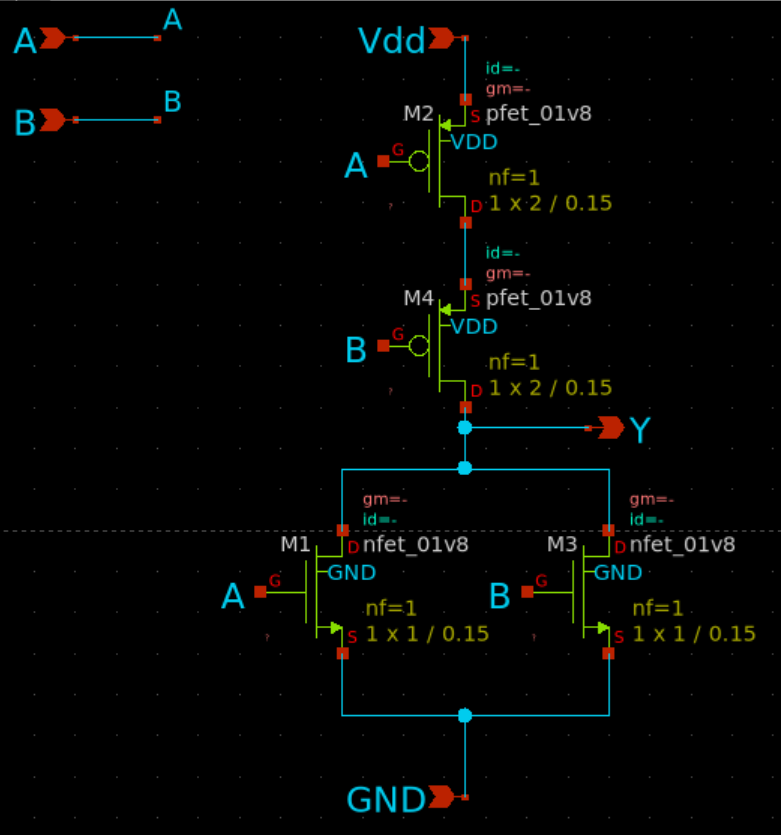
\includegraphics[width=0.4\textwidth]{nor_schematic.png}}
		\caption{NOR Circuit Schematic}
		\label{fig::nor_schematic}
	\end{figure}
	
	We also create a circuit symbol for the NOR gate, which is shown in Figure \ref{fig::nor_symbol}.
	
	\begin{figure}[H]
		\centerline{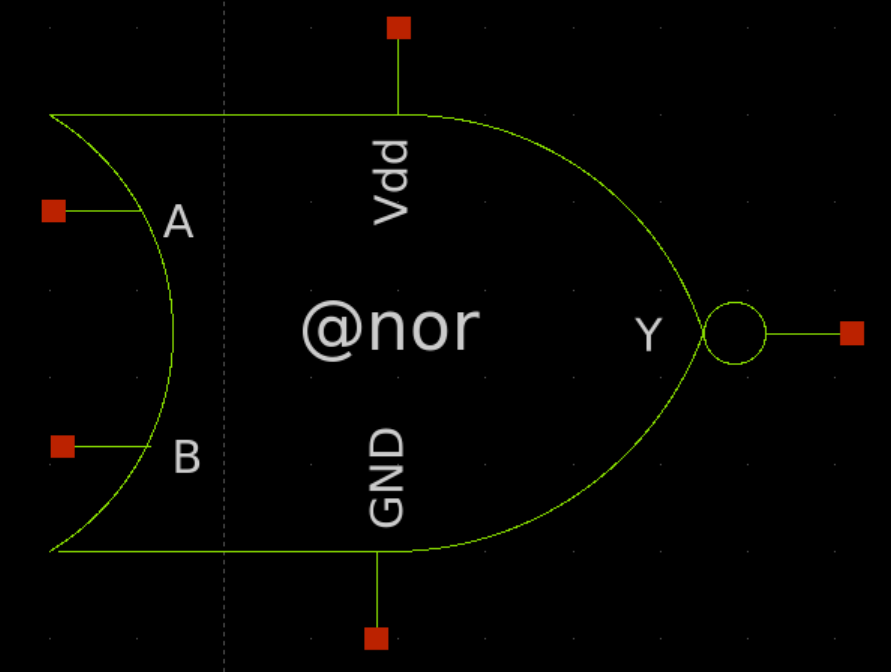
\includegraphics[width=0.4\textwidth]{nor_symbol.png}}
		\caption{NOR Circuit Symbol}
		\label{fig::nor_symbol}
	\end{figure}

	\subsubsection{Voltage Transfer Characteristics}
	
	In this section, we analyze the voltage transfer characteristics (VTC) of our NOR gate. For this analysis, we analyze the VTC when varying \texttt{a} and \texttt{b} independently and when varying \texttt{a} and \texttt{b} together. The test circuit we use when just varying the input \texttt{a} is included in Figure \ref{fig::nor_vtc_test_sweep_va}.
	
	\begin{figure}[H]
		\centerline{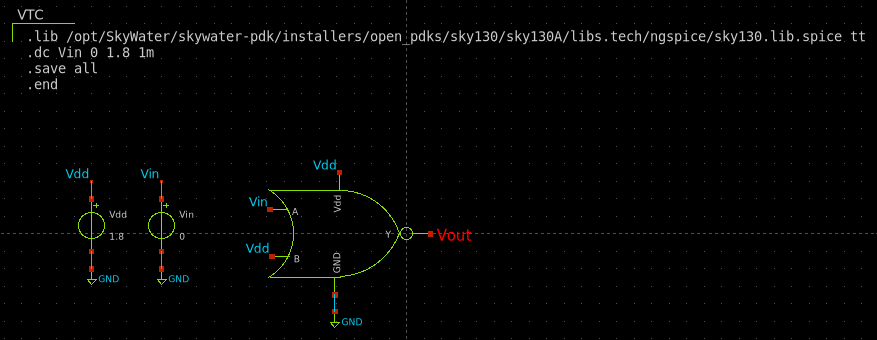
\includegraphics[width=0.8\textwidth]{nor_vtc_test_sweep_va.png}}
		\caption{NOR VTC Test Circuit for Independent Variations of Input \texttt{a}}
		\label{fig::nor_vtc_test_sweep_va}
	\end{figure}
	
	Using this test circuit, we perform DC analysis to determine the VTC and find \texttt{Va}, which is the voltage at which \texttt{Vin = Vout}. The results of this analysis are shown in Figure \ref{fig::nor_vtc_sweep_va}.
	
	\begin{figure}[H]
		\centerline{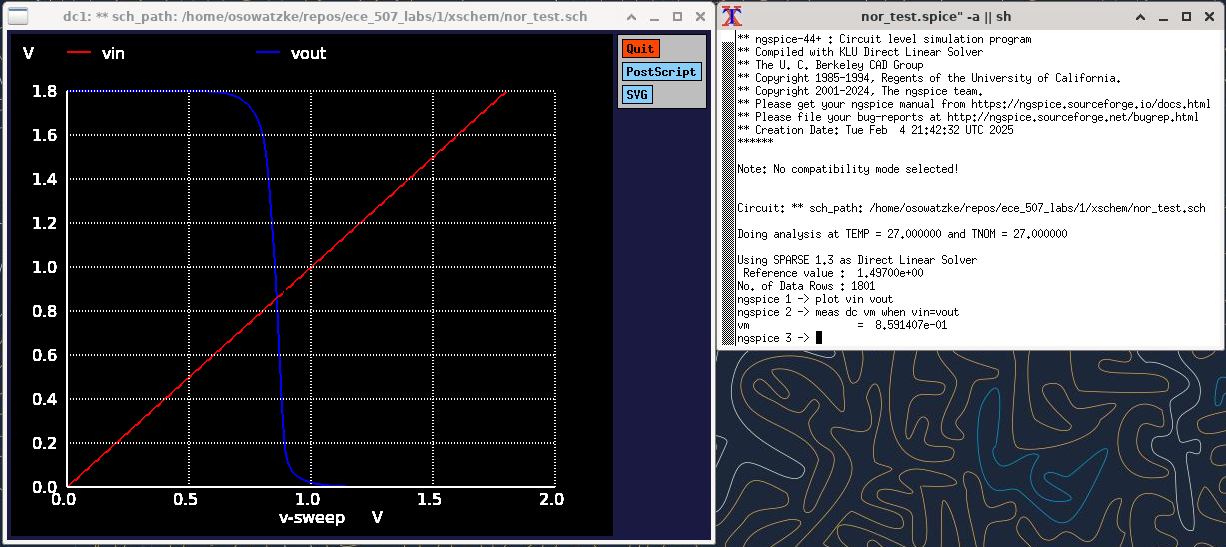
\includegraphics[width=0.8\textwidth]{nor_vtc_sweep_va.png}}
		\caption{NOR VTC Results for Independent Variations of Input \texttt{a}}
		\label{fig::nor_vtc_sweep_va}
	\end{figure}
	
	Examining the results, we find that \texttt{Vm = 0.8591V}. We perform similar analysis for independent variations of the input \texttt{b}. The test circuit and results are attached in figures \ref{fig::nor_vtc_test_sweep_vb} and \ref{fig::nor_vtc_sweep_vb} independently.
	
	\begin{figure}[H]
		\centerline{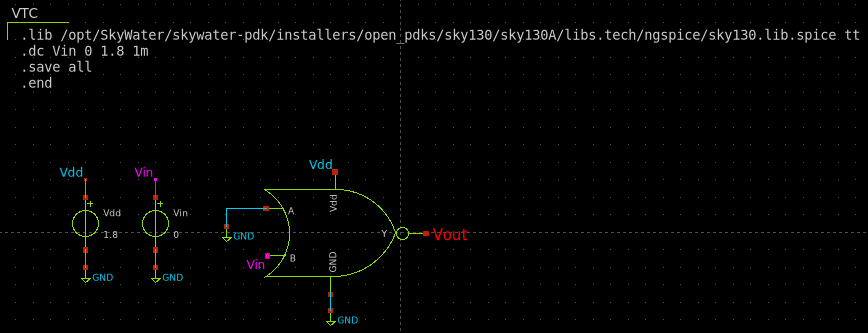
\includegraphics[width=0.8\textwidth]{nor_vtc_test_sweep_vb.png}}
		\caption{NOR VTC Test Circuit for Independent Variations of Input \texttt{b}}
		\label{fig::nor_vtc_test_sweep_vb}
	\end{figure}
	
	\begin{figure}[H]
		\centerline{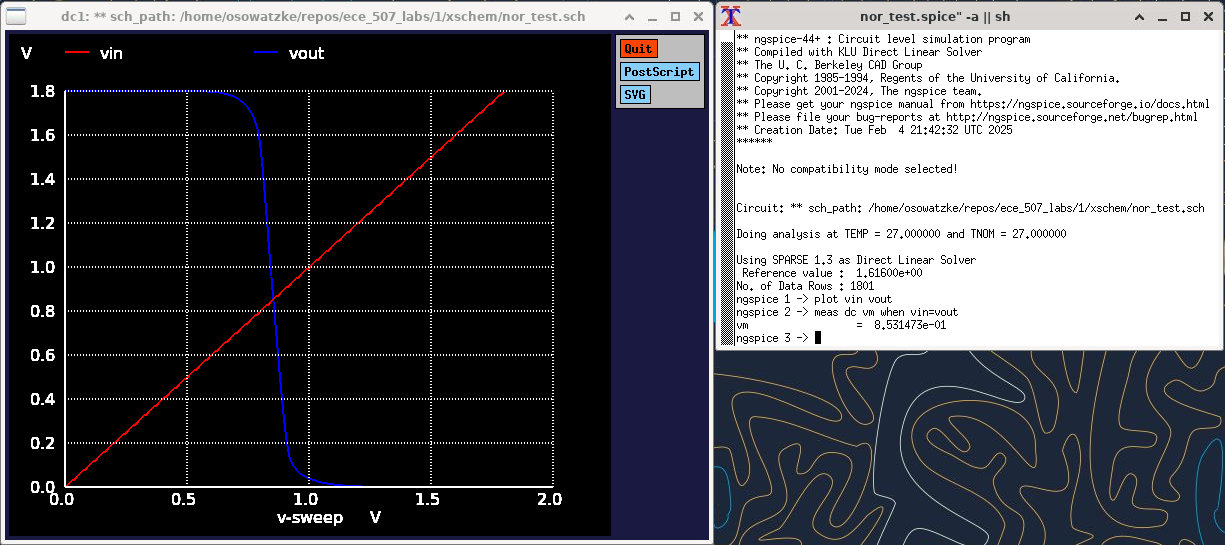
\includegraphics[width=0.8\textwidth]{nor_vtc_sweep_vb.png}}
		\caption{NOR VTC Results for Independent Variations of Input \texttt{b}}
		\label{fig::nor_vtc_sweep_vb}
	\end{figure}
	
	Examining the results, we find that \texttt{Vm = 0.8531V}. Finally, we sweep both inputs \texttt{a} and \texttt{b} together. The test circuit and results for this analysis are included in Figures \ref{fig::nor_vtc_test_sweep_va_vb} and \ref{fig::nor_vtc_sweep_va_vb} respectively.
	
	\begin{figure}[H]
		\centerline{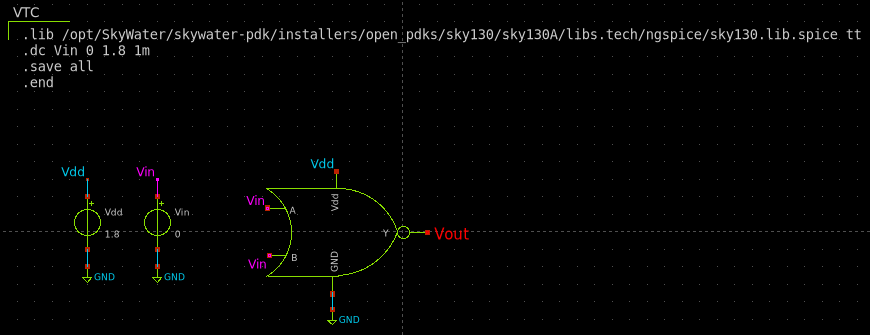
\includegraphics[width=0.8\textwidth]{nor_vtc_test_sweep_va_vb.png}}
		\caption{NOR VTC Test Circuit for Joint Variations of Inputs \texttt{a} and \texttt{b}}
		\label{fig::nor_vtc_test_sweep_va_vb}
	\end{figure}
	
	\begin{figure}[H]
		\centerline{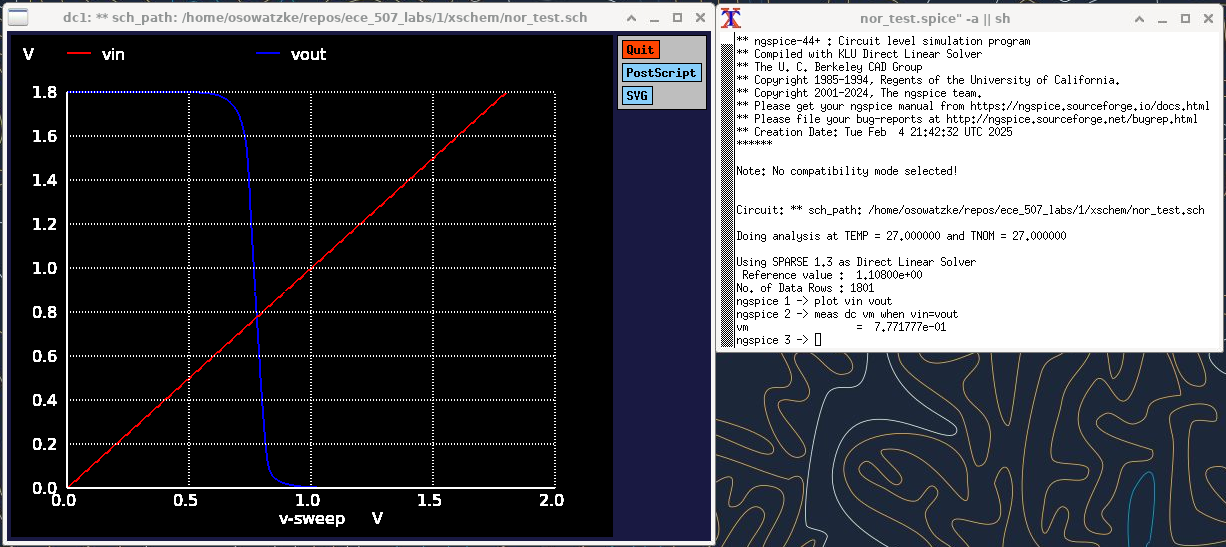
\includegraphics[width=0.8\textwidth]{nor_vtc_sweep_va_vb.png}}
		\caption{NOR VTC Results for Joint Variations of Inputs \texttt{a} and \texttt{b}}
		\label{fig::nor_vtc_sweep_va_vb}
	\end{figure}
	
	Examining the results, we find that \texttt{Vm = 0.7772V}.
	
	\subsubsection{Noise Analysis}
	
	In this section, we perform noise analysis of the NOR circuit following the process outlined for the NAND gate in Section \ref{section::nand_noise_analysis}. For this analysis, we use the test circuits shown in Figures \ref{fig::nor_vtc_test_sweep_va}, \ref{fig::nor_vtc_test_sweep_vb}, and \ref{fig::nor_vtc_test_sweep_va_vb}. We specifically use the test circuits to measure the noise margins, which are defined in Equations \ref{eq::noise_margin_high} and \ref{eq::noise_margin_low}. For the case in which we only vary the input \texttt{a}, we can identify the unity gain points ($V_{IH}$ and $V_{IL}$) and the corresponding noise margins as follows:
	
	\begin{figure}[H]
		\centerline{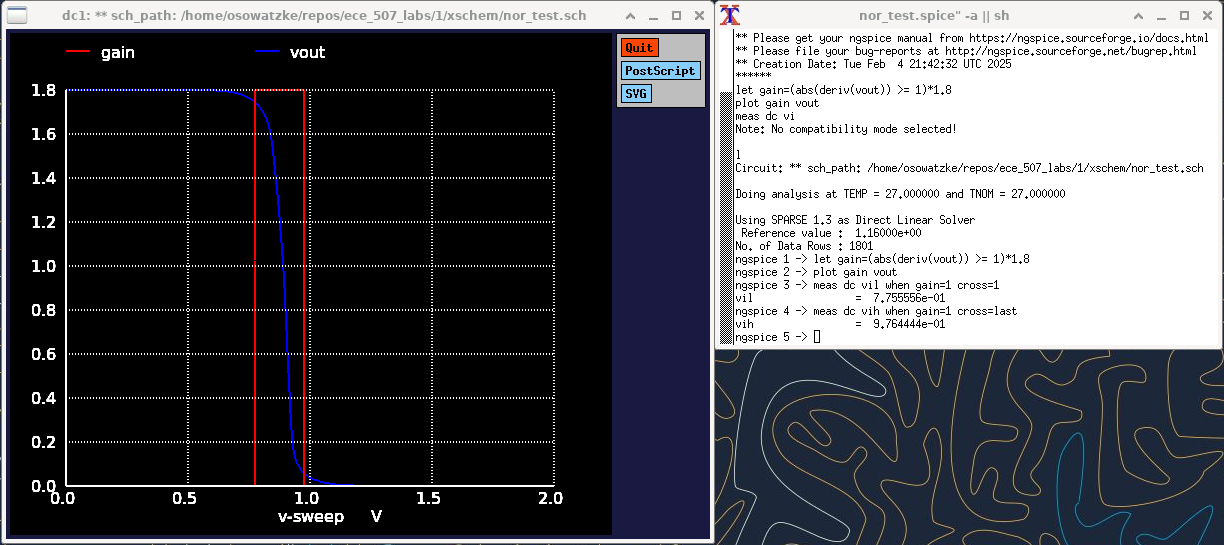
\includegraphics[width=0.8\textwidth]{nor_noise_analysis_sweep_va.png}}
		\caption{Measuring \texttt{Vil} for the NOR Gate when Input Variations are Limited to Input \texttt{a}}
		\label{fig::nor_noise_analysis_sweep_va}
	\end{figure}
	
	Examining the ngspice outputs, we find that \texttt{Vil = 0.7336 V} and \texttt{Vih = 0.9354 V}. This implies that \texttt{Nmh = 1.8 V - 0.9354 V = 0.8646 V} and \texttt{Nml = 0.7336 V}. We can repeat this analysis for independent variations of the input \texttt{b} and for joint variations of inputs \texttt{a} and \texttt{b}. The ngspice outputs for this analysis are included in Figure \ref{fig::nor_noise_analysis_sweep_vb} and \ref{fig::nor_noise_analysis_sweep_va_vb}.
	
	\begin{figure}[H]
		\centerline{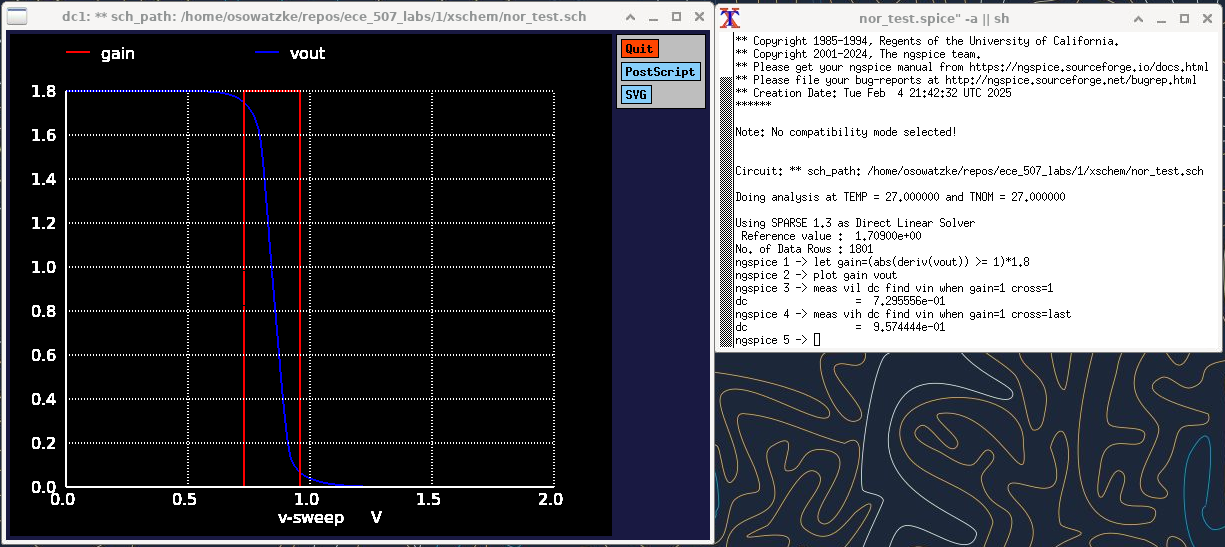
\includegraphics[width=0.8\textwidth]{nor_noise_analysis_sweep_vb.png}}
		\caption{Measuring \texttt{Vil} for the NOR Gate when Input Variations are Limited to Input \texttt{b}}
		\label{fig::nor_noise_analysis_sweep_vb}
	\end{figure}
	
	\begin{figure}[H]
		\centerline{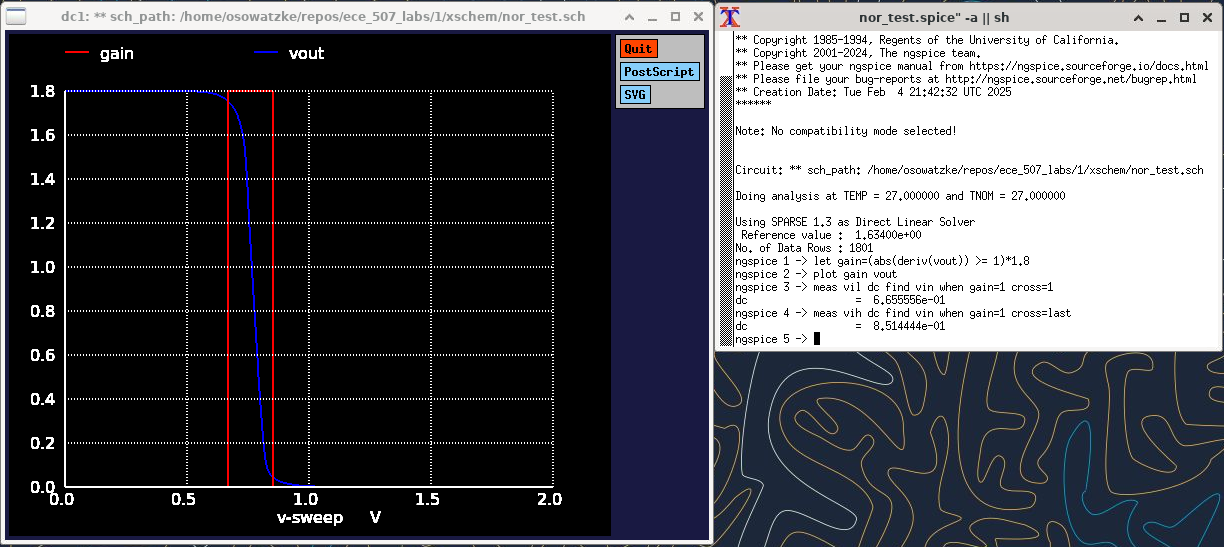
\includegraphics[width=0.8\textwidth]{nor_noise_analysis_sweep_va_vb.png}}
		\caption{Measuring \texttt{Vil} for the NOR Gate when Inputs \texttt{a} and \texttt{b} are Varied Together}
		\label{fig::nor_noise_analysis_sweep_va_vb}
	\end{figure}
	
	Examining the outputs, we find that the noise margins are defined as \texttt{Nmh = 0.8426 V} and \texttt{Nml = 0.7296 V} when input variations are limited to input \texttt{b}. When we vary the inputs \texttt{a} and \texttt{b} in unison, we find that the noise margins are \texttt{Nmh = 0.9486 V} and \texttt{Nml = 0.6656 V}.
	
	\subsubsection{Delay Analysis}
	
	In this section, we analyze the delay of the NOR gate by measuring the high to low propagation delay (\texttt{tphl}). To perform this analysis for independent variations of the input \texttt{a}, we use the following test circuit:
	
	\begin{figure}[H]
		\centerline{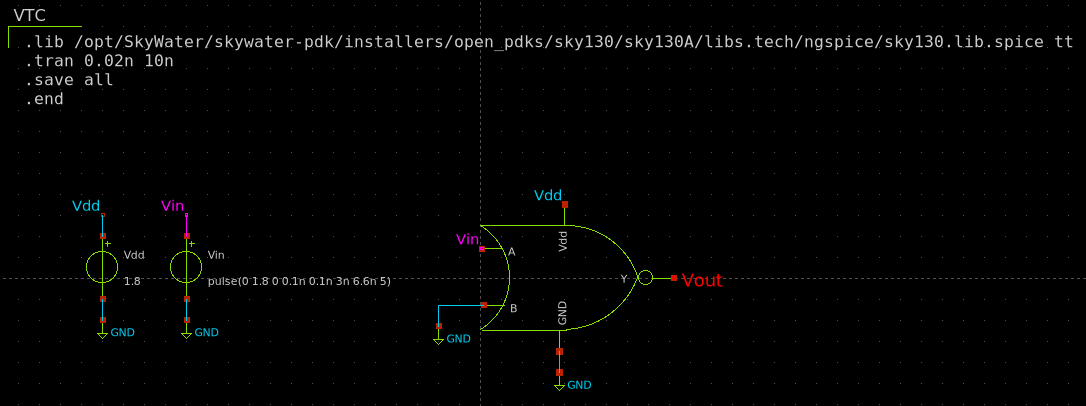
\includegraphics[width=0.8\textwidth]{nor_delay_test_sweep_va.png}}
		\caption{Test Circuit to Measure the Delay of the NOR Gate when Only Input \texttt{a} is Varied}
		\label{fig::nor_delay_test_sweep_va}
	\end{figure}
	
	Using the test circuit, we measure can measure the high-to-low propagation delay as follows:
	
	\begin{figure}[H]
		\centerline{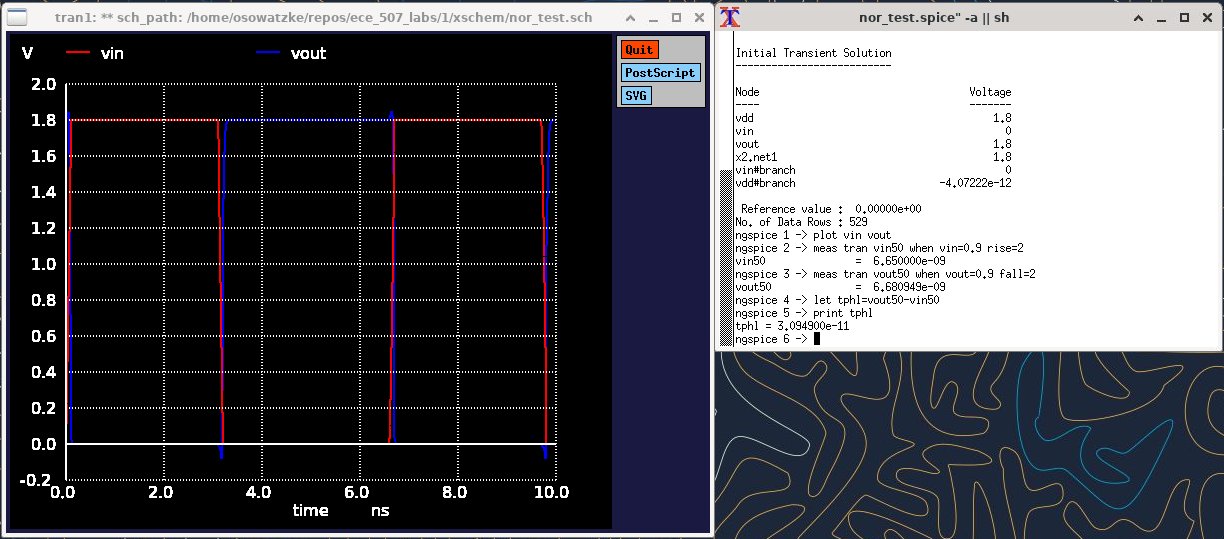
\includegraphics[width=0.8\textwidth]{nor_delay_sweep_va.png}}
		\caption{\texttt{tphl} Measurement for the NOR Gate when Input Variations are Limited to Input \texttt{a}}
		\label{fig::nor_delay_sweep_va}
	\end{figure}
	
	Examining the output results, we find that \texttt{tphl = 30.949 ps}. We can perform similar analysis to examine the impact of varying just the input \texttt{b}. The test circuits for this analysis is shown in Figures \ref{fig::nor_delay_test_sweep_vb} and the results are shown in Figure \ref{fig::nor_delay_sweep_vb}.
	
	\begin{figure}[H]
		\centerline{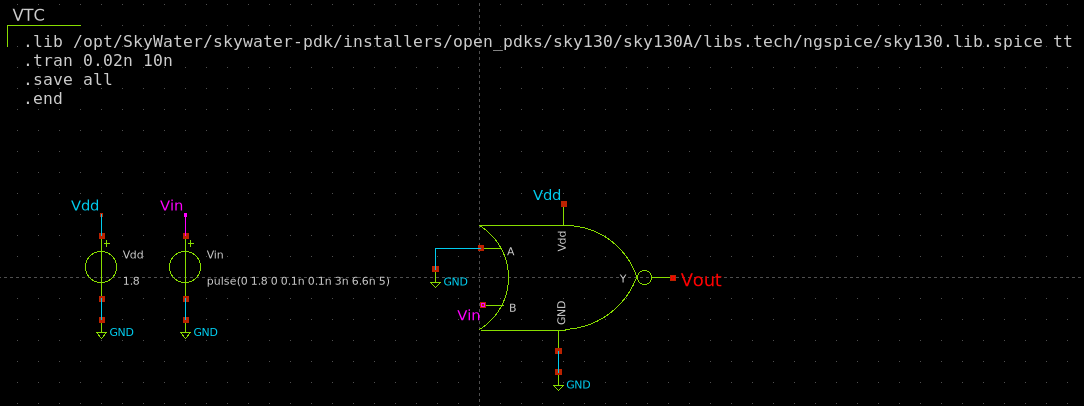
\includegraphics[width=0.8\textwidth]{nor_delay_test_sweep_vb.png}}
		\caption{Test Circuit to Measure the Delay of the NOR Gate when Only Input \texttt{b} is Varied}
		\label{fig::nor_delay_test_sweep_vb}
	\end{figure}
	
	\begin{figure}[H]
		\centerline{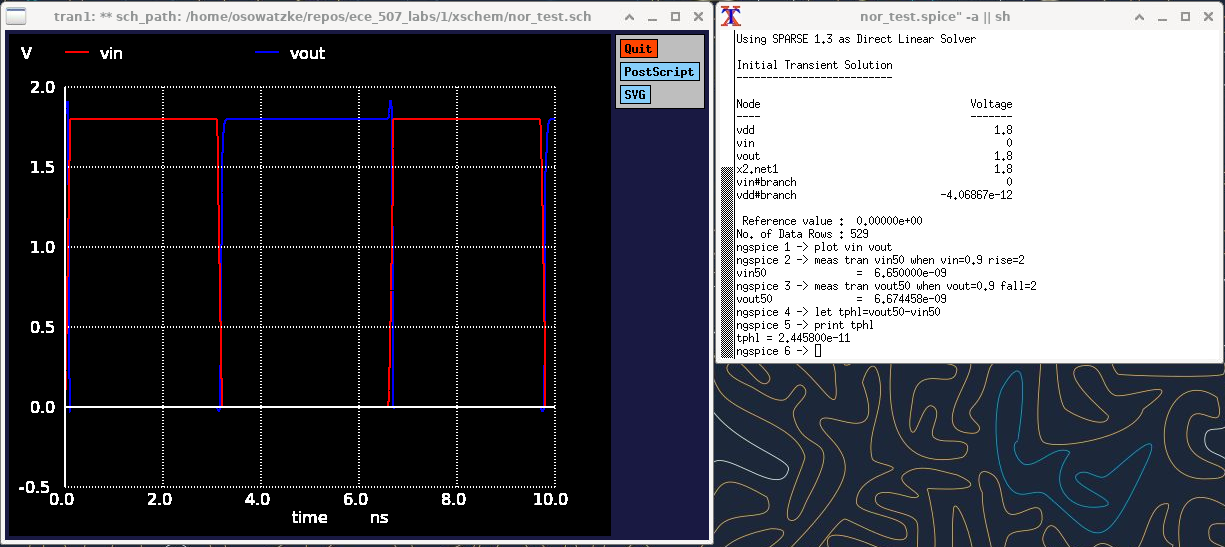
\includegraphics[width=0.8\textwidth]{nor_delay_sweep_vb.png}}
		\caption{\texttt{tphl} Measurement for the NOR Gate when Input Variations are Limited to Input \texttt{b}}
		\label{fig::nor_delay_sweep_vb}
	\end{figure}
	
	Examining the output results, we find that \texttt{tphl = 24.458 ps}. Finally, we can examine the impact of varying both inputs together. The test circuit for this analysis is shown in Figure  \ref{fig::nor_delay_test_sweep_va_vb} and the results are captured in Figure  \ref{fig::nor_delay_sweep_va_vb}.
	
	\begin{figure}[H]
		\centerline{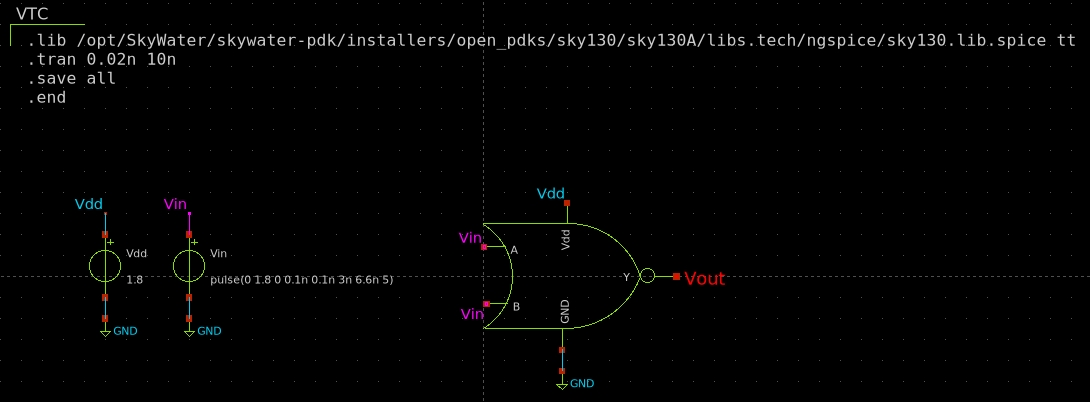
\includegraphics[width=0.8\textwidth]{nor_delay_test_sweep_va_vb.png}}
		\caption{Test Circuit to Measure the Delay of the NOR Gate when Both Inputs are Varied Together}
		\label{fig::nor_delay_test_sweep_va_vb}
	\end{figure}
	
	\begin{figure}[H]
		\centerline{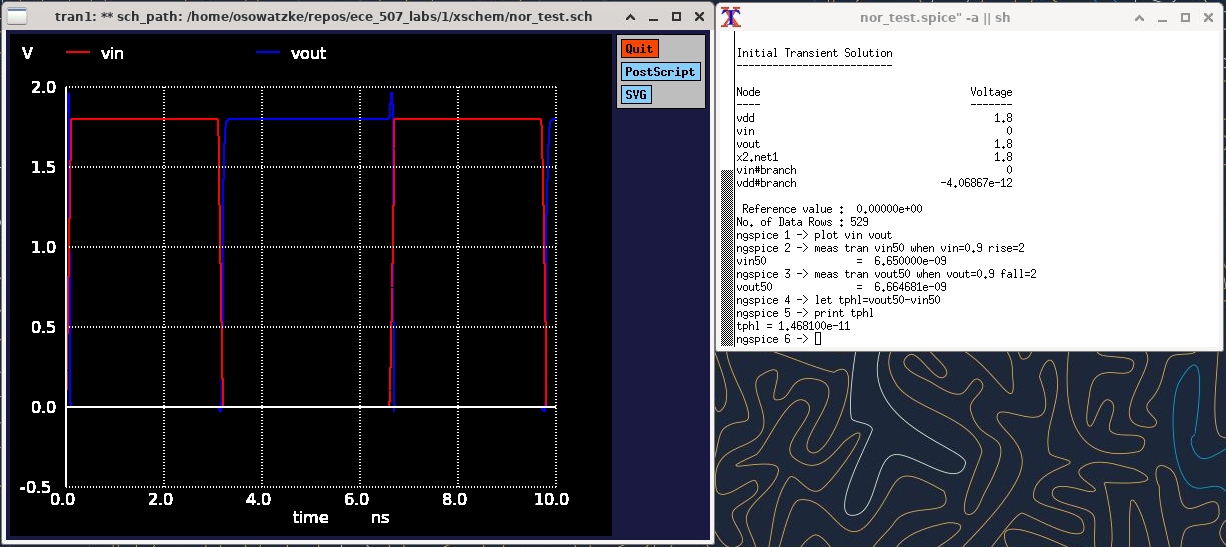
\includegraphics[width=0.8\textwidth]{nor_delay_sweep_va_vb.png}}
		\caption{\texttt{tphl} Measurement for the NOR Gate when Both Inputs are Varied Together}
		\label{fig::nor_delay_sweep_va_vb}
	\end{figure}
	
	Examining the output, we find that \texttt{tphl=14.681 ps}. Note that the delays are data dependent.
	
	\subsubsection{Power Analysis}
	
	In this section, we analyze the power consumption of our NOR gate. Our test circuit for this analysis is included in Figure \ref{fig::nor_power_test_sweep_va}, and the results of our analysis are shown in Figure \ref{fig::nor_power_sweep_va}.
	
	\begin{figure}[H]
		\centerline{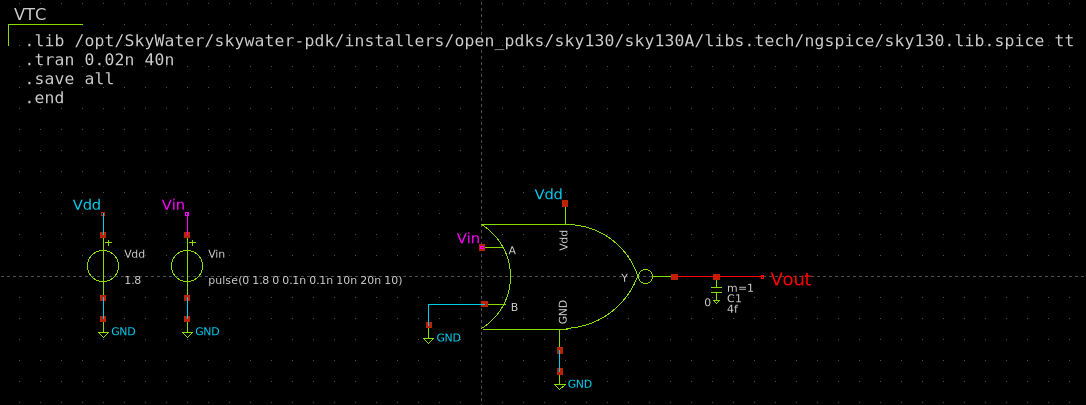
\includegraphics[width=0.8\textwidth]{nor_power_test_sweep_va.png}}
		\caption{Test Circuit to Measure the Power Consumption of the NOR Gate when \texttt{b=1} and Input \texttt{a} is Varied}
		\label{fig::nor_power_test_sweep_va}
	\end{figure}
	
	\begin{figure}[H]
		\centerline{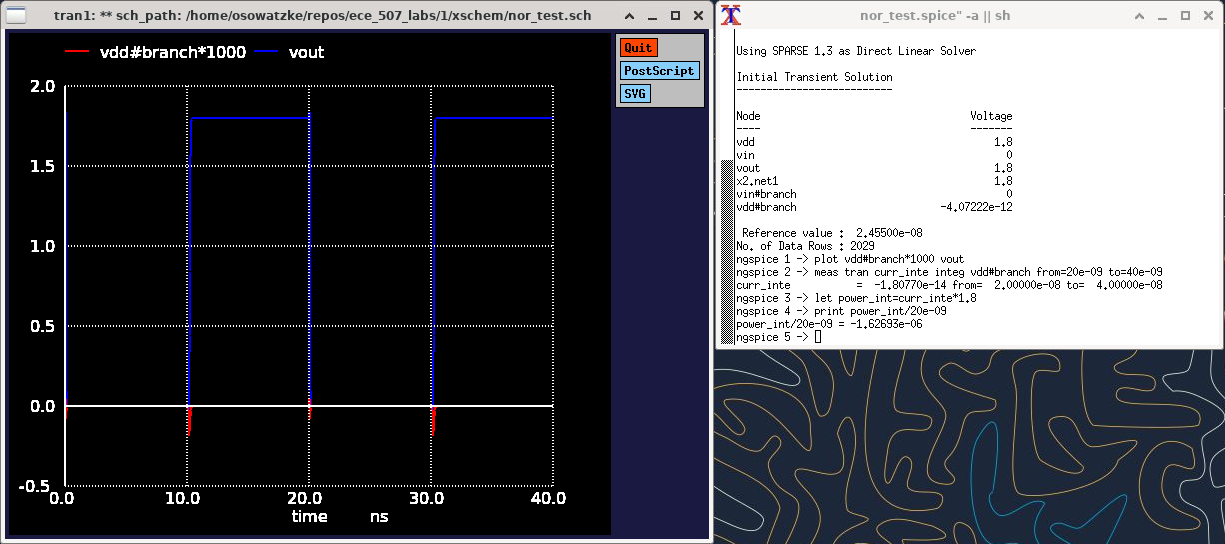
\includegraphics[width=0.8\textwidth]{nor_power_sweep_va.png}}
		\caption{Power Consumption of the NOR Gate when \texttt{b=1} and Input \texttt{a} is Varied}
		\label{fig::nor_power_sweep_va}
	\end{figure}
	
	Examining the results, we find that the power consumption is $1.62693{\mu}W$. We can also measure the power consumption when we fix \texttt{a} at 1 and vary \texttt{b}. The test circuit for this analysis is shown in Figure \ref{fig::nor_power_test_sweep_vb} and the results are shown in Figure \ref{fig::nor_power_sweep_vb}.
	
	\begin{figure}[H]
		\centerline{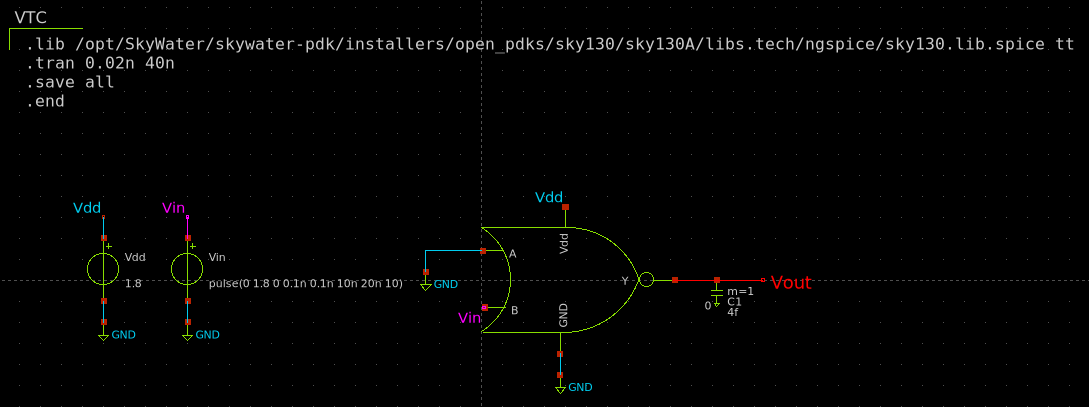
\includegraphics[width=0.8\textwidth]{nor_power_test_sweep_vb.png}}
		\caption{Test Circuit to Measure the Power Consumption of the NOR Gate when \texttt{a=1} and Input \texttt{b} is Varied}
		\label{fig::nor_power_test_sweep_vb}
	\end{figure}
	
	\begin{figure}[H]
		\centerline{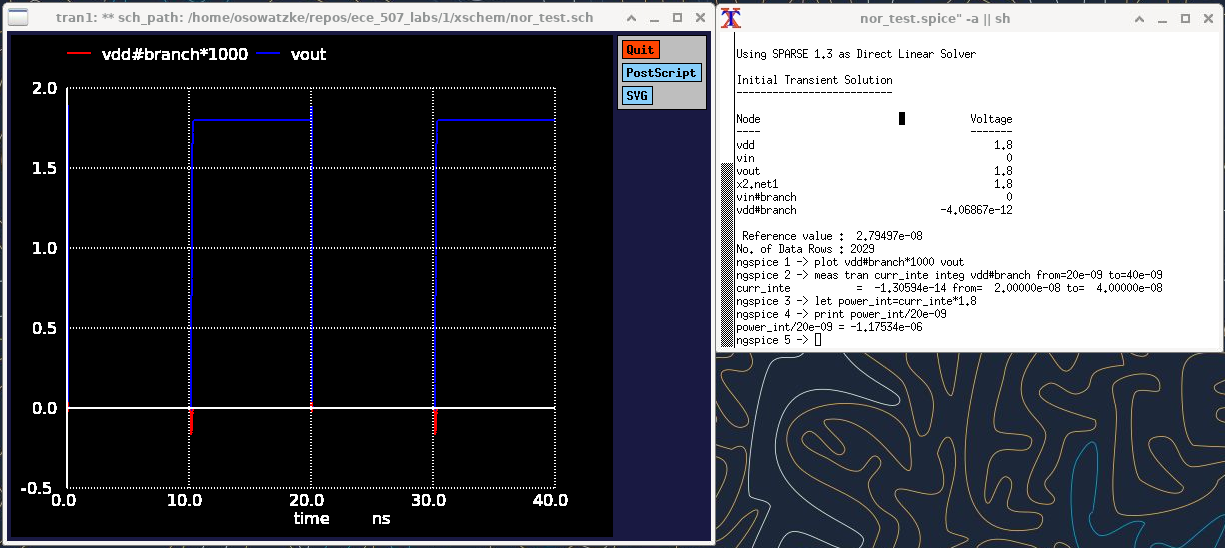
\includegraphics[width=0.8\textwidth]{nor_power_sweep_vb.png}}
		\caption{Power Consumption of the NOR Gate when \texttt{a=1} and Input \texttt{b} is Varied}
		\label{fig::nor_power_sweep_vb}
	\end{figure}
	
	Examining the results, we find that the power consumption is $1.17534{\mu}W$. Next, we measure the power when the inputs are varied together. For this analysis, we use the test circuit shown in Figure \ref{fig::nor_power_test_sweep_va_vb}.
	
	\begin{figure}[H]
		\centerline{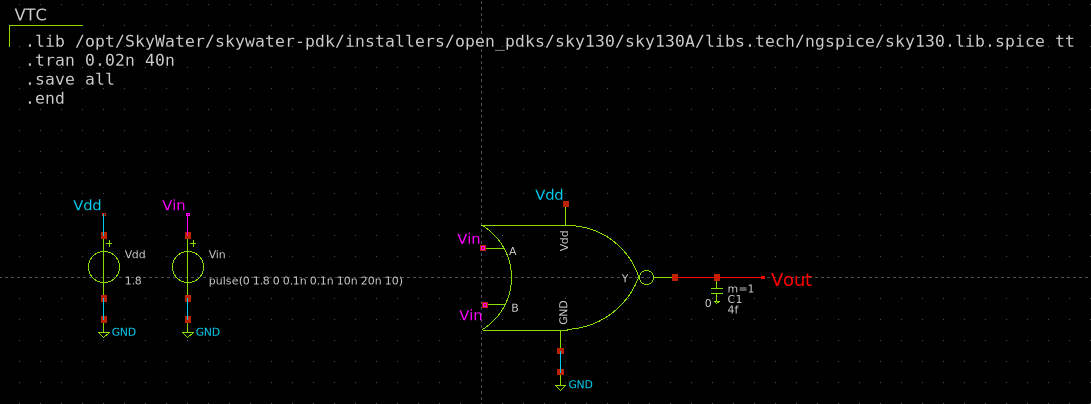
\includegraphics[width=0.8\textwidth]{nor_power_test_sweep_va_vb.png}}
		\caption{Test Circuit to Measure the Power Consumption of the NOR Gate when Both Inputs are Varied Together}
		\label{fig::nor_power_test_sweep_va_vb}
	\end{figure}
	
	The results of our analysis are included in Figure \ref{fig::nor_power_sweep_va_vb} and indicate a power consumption of $1.31831{\mu}W$. 
	
	\begin{figure}[H]
		\centerline{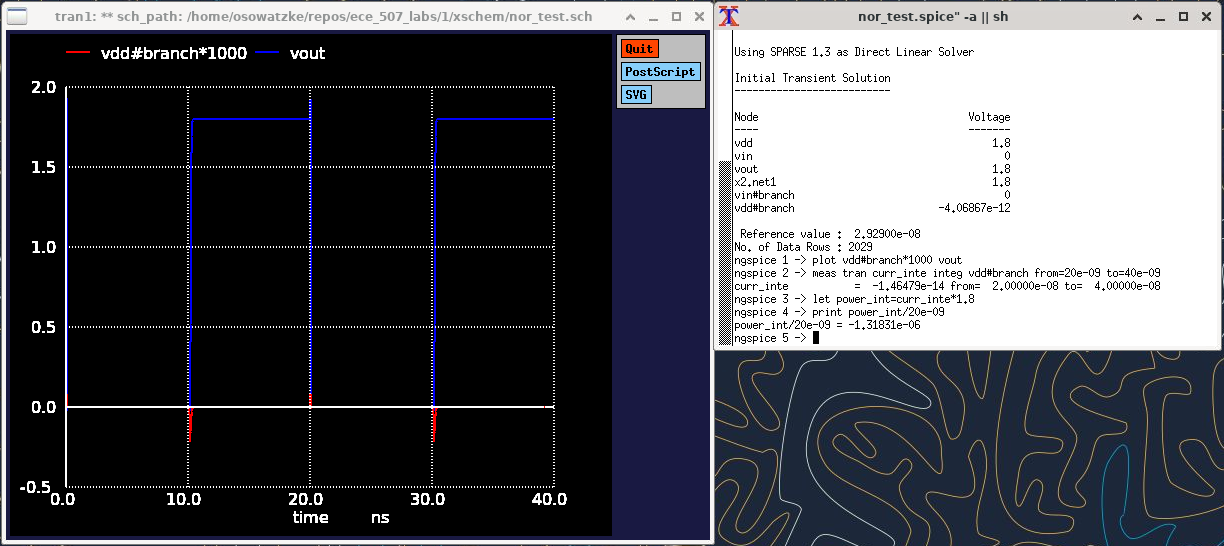
\includegraphics[width=0.8\textwidth]{nor_power_sweep_va_vb.png}}
		\caption{Power Consumption of the NOR Gate when Both Inputs are Varied Together}
		\label{fig::nor_power_sweep_va_vb}
	\end{figure}	
	
	\subsection{NAND Gate}

	\begin{align}
		I_{ds_p} &= -k_p\frac{W_p}{L}V_{dsat_p}\left(V_{gs_p} - V_{T0_p} - \frac{V_{dsat_p}}{2}\right)\left(1 + {\lambda_p}V_{ds_p}\right) \\
		&= -k_p\frac{W}{L}V_{dsat_p}\left(V_m - V_{dd} - V_{T0_p} - \frac{V_{dsat_p}}{2}\right)\left(1 + {\lambda_p}(V_m - V_{dd})\right)
	\end{align}
	
	\begin{align}
		I_{ds_n} &= k_n\frac{W_n}{L}V_{dsat_n}\left(V_{gs_n} - V_{T0_n} - \frac{V_{dsat_n}}{2}\right)\left(1 + {\lambda_n}V_{ds_n}\right) \\
		&= k_n\frac{W_n}{L}V_{dsat_n}\left(V_m - V_{T0_n} - \frac{V_{dsat_n}}{2}\right)\left(1 + {\lambda_n}V_m\right)
	\end{align}
	
	Using KCL, we know that:
	
	\begin{equation}
		I_{ds_n} + I_{ds_p} = 0
	\end{equation}
	
	Solving numerically, using the parameters in Table \ref{table::nmos_params} we find that $V_m = 0.8422 V$.
	
	
\end{document}